\documentclass[notes,10pt, aspectratio=169]{beamer}

\usepackage{pgfpages}
% These slides also contain speaker notes. You can print just the slides,
% just the notes, or both, depending on the setting below. Comment out the want
% you want.
\setbeameroption{hide notes} % Only slide
%\setbeameroption{show only notes} % Only notes
%\setbeameroption{show notes on second screen=right} % Both

\usepackage{helvet}
\usepackage[default]{lato}
\usepackage{array}
\usepackage{eurosym}
\usepackage{setspace}
\usepackage{animate}
\usepackage{multicol}
\usepackage{breqn}
\usepackage{subcaption}
\usepackage{caption}
\captionsetup{font=scriptsize, justification=raggedright,singlelinecheck=false}
\usepackage[export]{adjustbox}
\usepackage[scale=2]{ccicons}
\usepackage{tikz}
\newenvironment{wideitemize}{\itemize\addtolength{\itemsep}{10pt}}{\enditemize}
\usepackage{natbib}

\usepackage{tikz}
\usepackage{verbatim}
\setbeamertemplate{note page}{\pagecolor{yellow!5}\insertnote}
\usepackage{amsmath}
%\usepackage{mathpazo}
\usepackage{hyperref}
\usepackage{lipsum}
\usepackage{multimedia}
\usepackage{multirow}
\usepackage{graphicx}
\usepackage{dcolumn}
\usepackage{bbm}
\newcolumntype{d}[0]{D{.}{.}{5}}

\usepackage{changepage}
\usepackage{appendixnumberbeamer}
% \newcommand{\beginbackup}{
%   \newcounter{framenumbervorappendix}
%   \setcounter{framenumbervorappendix}{\value{framenumber}}
%   \setbeamertemplate{footline}
%   {
%      \leavevmode%
%      \hline
%      box{%
%       \begin{beamercolorbox}[wd=\paperwidth,ht=2.25ex,dp=1ex,right]{footlinecolor}%
% %         \insertframenumber  \hspace*{2ex} 
%       \end{beamercolorbox}}%
%      \vskip0pt%
%   }
%  }

 \setbeamertemplate{footline}{
    \hbox{%
    \begin{beamercolorbox}[wd=\paperwidth,ht=3ex,dp=1.5ex,leftskip=2ex,rightskip=2ex]{page footer}%
        %\usebeamerfont{title in head/foot}%
        %\insertshorttitle \hfill
        %\insertsection \hfill
        %\tableofcontents[currentsection] \hfill
        \insertsectionnavigationhorizontal{0.7\paperwidth}{}{} \hfill 
        \insertframenumber{} / \inserttotalframenumber
    \end{beamercolorbox}}%
}
\newcommand{\backupend}{
   \addtocounter{framenumbervorappendix}{-\value{framenumber}}
   \addtocounter{framenumber}{\value{framenumbervorappendix}} 
}


\usepackage{graphicx}
\usepackage[space]{grffile}
\usepackage{booktabs}

% These are my colors -- there are many like them, but these ones are mine.
\definecolor{blue}{RGB}{0,114,178}
\definecolor{red}{RGB}{213,94,0}
\definecolor{yellow}{RGB}{240,228,66}
\definecolor{green}{RGB}{0,158,115}

\setbeamercolor{section in head/foot}{fg=blue}

\useinnertheme[shadow]{rounded}
\setbeamercolor{block title example}{fg=black,bg=orange!50!white}
\setbeamercolor{block body example}{fg=black, bg=orange!30!white}


\hypersetup{
  colorlinks=false,
  linkbordercolor = {white},
  linkcolor = {blue}
}


%% I use a beige off white for my background
\definecolor{MyBackground}{RGB}{255,253,218}

%% Uncomment this if you want to change the background color to something else
%\setbeamercolor{background canvas}{bg=MyBackground}

%% Change the bg color to adjust your transition slide background color!
\newenvironment{transitionframe}{
  \setbeamercolor{background canvas}{bg=yellow}
  \begin{frame}}{
    \end{frame}
}

\setbeamercolor{frametitle}{fg=blue}
\setbeamercolor{title}{fg=black}
%\setbeamertemplate{footline}[frame number]
\setbeamertemplate{navigation symbols}{} 
\setbeamertemplate{itemize items}{-}
\setbeamercolor{itemize item}{fg=blue}
\setbeamercolor{itemize subitem}{fg=blue}
\setbeamercolor{enumerate item}{fg=blue}
\setbeamercolor{enumerate subitem}{fg=blue}
\setbeamercolor{button}{bg=white,fg=blue,}



% If you like road maps, rather than having clutter at the top, have a roadmap show up at the end of each section 
% (and after your introduction)
% Uncomment this is if you want the roadmap!
% \AtBeginSection[]
% {
%    \begin{frame}
%        \frametitle{Roadmap of Talk}
%        \tableofcontents[currentsection]
%    \end{frame}
% }
\setbeamercolor{section in toc}{fg=blue}
\setbeamercolor{subsection in toc}{fg=red}
%\setbeamersize{text margin left=1em,text margin right=1em} 
\setbeamersize{text margin left=0.7cm,text margin right=0.7cm} 


\title[]{\textcolor{blue}{Lecture 1:\\Introduction and Review of Probability}}
\author{25117 - Econometrics}
\institute[shortinst]{Universitat Pompeu Fabra}

%\date{September 25th, 2024}

\begin{document}



% Title Slide

\begin{frame}[plain]
\maketitle
\end{frame}

\section{Introduction}

\begin{frame}[label=intro_0]{About this course}
%\underline{\textbf{\large Metadata:}}\\
%\begin{itemize}
%    \item[--] \textit{Teacher:}~~~~~~~~~~~~~ Pierre Magontier
%    \item[--] \textit{Office:}~~~~~~~~~~~~~~~~ 20.1.E50
%    \item[--] \textit{Email:} ~~~~~~~~~~~~~~~~~pierre.magontier@upf.edu
%    \item[--] \textit{Office hour:} ~~~~~~~~ Wednesdays, 2pm-3pm
%    \item[--] \textit{Material:} ~~~~~~~~~~~~~Aula Global
%    \item[--] \textit{Main Readings:}    \begin{itemize}
%        \item[\longrightarrow] Lecture notes
%        \item[\longrightarrow] Introduction to Econometrics, Global Edition, 4th edition, Stock and Watson
%    \end{itemize}
%\end{itemize}

\vspace{.3cm}
\underline{\textbf{\large Evaluation:}}\\
\begin{itemize}
    \item[--] \textit{\color{teal}{Problem Sets (Seminars)}} x 10\% +  \textit{\color{orange}{Mid-term Exam:}} x 30\% + \textit{\color{purple}{Final Exam:}} x 60\% 
\end{itemize}

\end{frame}


\begin{frame}{What's Econometrics about?}
    \begin{itemize}
        \item[-] Economics is the social science that studies how economic agents (i.e., individuals, businesses, governments, societies, etc.) allocate scarce resources (e.g., time, money, etc.) to satisfy an objective.\vspace{.2cm}
        \item[-] Resulting allocation choices matter --- \textit{"There is no free lunch!"}  --- as they suggest important relationships (e.g., "Education matters for future income/personal well-being/etc.")\vspace{.2cm}
        \item[-] Econometrics is a specialized branch of economics that focuses on the application of statistical methods to analyze and quantify these economic relationships.\vspace{.2cm}
        \begin{itemize}
            \item[$\rightarrow$] How does another year of education change earnings?
            \item[$\rightarrow$]  What is the quantitative effect of reducing class size on student achievement?
            \item[$\rightarrow$] What is the effect on housing prices of environmental improvements?
        \end{itemize}\vspace{.2cm}
        \item[-] Goal: To bridge the gap between economic theory and real-world data by using empirical evidence to test and refine economic theories.
    \end{itemize}
\end{frame}


\begin{frame}{Inferring Causal Effects (and more)}
    \begin{itemize}
         \item[-] In most applied econometrics problems, we seek to identify the causal effect of a change in a treatment variable $D$ on an outcome $Y$.\vspace{.2cm}
         \item[-] Ideally, this would require a randomized control experiment: the treatment $D$ is randomly assigned to a sample population.\vspace{.2cm}
         \item[-] Randomization ensures that there are no systematic differences between the control (or comparison) and the treated groups.\vspace{.2cm}
         \item[-] Most of these experiments would be completely unethical (and if not, extremely costly) ! \vspace{.2cm}
        \item[-] Instead, we have to rely on observational (i.e., non-experimental) data, which might be jointly determined. How to identify causal effects, then?
    \end{itemize}
\end{frame}


\begin{frame}{A sentence you are going to hear a lot}
\begin{center}
      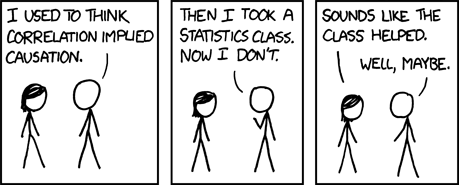
\includegraphics[scale=.9]{images/correlation.png}  
\end{center}
\end{frame}


\begin{frame}[label=intro_0]{Outline (Preliminary!)}
\begin{columns} 
% Column 1
    \begin{column}{.5\textwidth}
        \begin{center}
            \textbf{BLOCK 1}
        \end{center}
        \begin{enumerate}
            \item Introduction and Review of Probability
            \item Review of Statistics
            \item[~] {\color{teal}{Practice 1}}
            \item Simple Linear Regression
            \item OLS Implementation
            \item[~] {\color{teal}{Practice 2}}
            \item Multivariate Linear Regression
            \item Inference and Interpretation
            \item[~] {\color{teal}{Practice 3}}
            \item Q \& A
            \item[$\longrightarrow$] {\color{orange}{Mid-Term Exam}}
        \end{enumerate}
    \end{column}
% Column 2    
    \begin{column}{.5\textwidth}
        \begin{center}
            \textbf{BLOCK 2}
        \end{center}
        \begin{enumerate}
        \setcounter{enumi}{7}
            \item Functional Forms
            \item Threats to Identification
            \item[~] {\color{teal}{Practice 4}}
            \item Instrumental Variables
            \item Panel Data
            \item Binary Choice Models
            \item[~] {\color{teal}{Practice 5}}
            \item[~]
            \item[~]
            \item[~]
            \item[~]
            \item[$\longrightarrow$] {\color{purple}{Final Exam}}
        \end{enumerate}

    \end{column}
\end{columns}
\end{frame}

\section{Review of Probability Theory - Random Variables}
\begin{frame}{Some Revision}
    \begin{enumerate}
        \item A random variable is a mathematical concept used to describe and model uncertain events
        \begin{itemize}
            \item NB: A random variable isn't inherently "unpredictable"; it represents different values tied to uncertain outcomes, each with assigned probabilities
        \end{itemize} \vspace{.2cm}
        \item The mutually exclusive potential results of a random process are called the outcomes \vspace{.2cm}
        \item The set of all possible outcomes is called the sample space. A subset of the sample space is called an event. \vspace{.2cm}
        \item The probability distribution of a random variable, $X$, is the list of all possible values, $x$, of the variable and the probability that each value will occur, $Pr(X=x)$. These probabilities sum to 1.
        \begin{itemize}
            \item NB: We talk about probability density function for continuous random variables (p.d.f.)
        \end{itemize} \vspace{.2cm}
        \item The cumulative distribution function (c.d.f.) is the probability that the random variable is less than or equal to a particular value
    \end{enumerate}
\end{frame}


\begin{frame}{P.d.f. of a continuous random variable}
    \begin{center}
        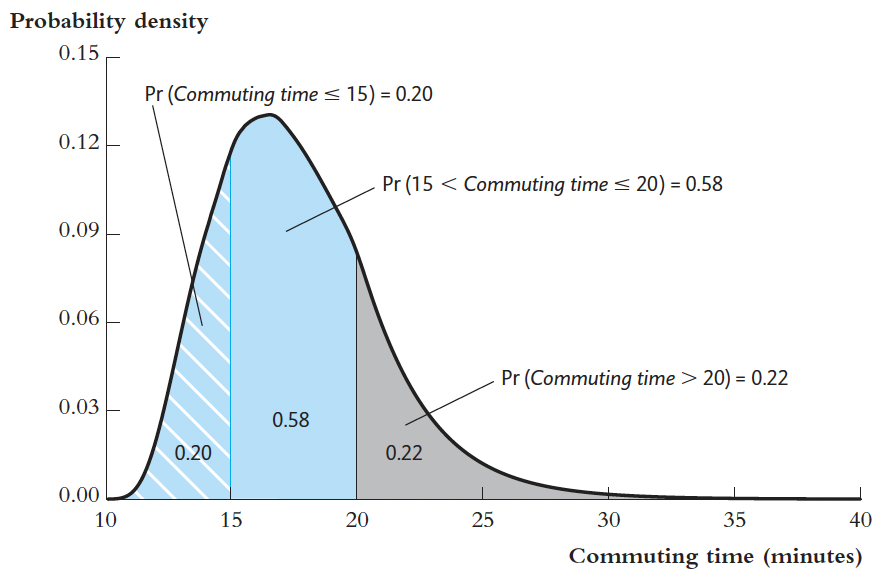
\includegraphics[scale=.7]{images/pdf.png}
    \end{center}
\end{frame}

\begin{frame}{C.d.f. of a continuous random variable}
    \begin{center}
        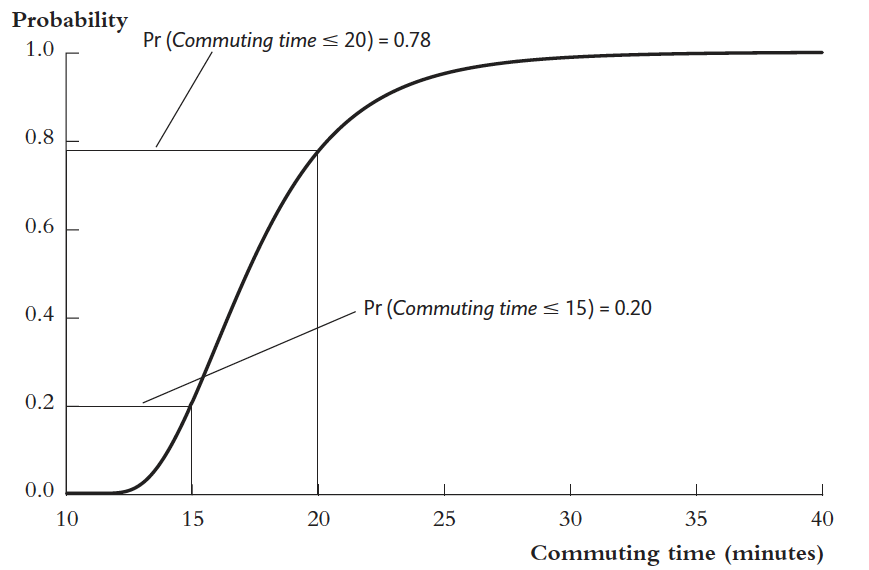
\includegraphics[scale=.7]{images/cdf.png}
    \end{center}
\end{frame}


\begin{frame}{Statistical Moments}
        \begin{enumerate}
            \item The mean (or expected value) indicates the long-run average of a random variable $Y$:
            \begin{equation*}
                \mathbb{E}(Y)\equiv\mu_Y = \sum^k_{i=1} y_iPr(Y=y_i)
            \end{equation*}
            \item The standard deviation (resp., variance) informs about the (resp., squared) dispersion of $Y$:
            \begin{equation*}
                \sigma^2_Y \equiv var(Y) = \mathbb{E}[(Y-\mu_Y)^2]= \sum^k_{i=1}(y_i-\mu_Y)^2Pr(Y=y_i)
            \end{equation*}
            \item The skewness informs about the asymmetry of $Y$:
            \begin{equation*}
                \gamma_Y = \mathbb{E}[(Y-\mu_Y)^3]\sigma_Y^{-3}
            \end{equation*}
            \item The kurtosis of $Y$ is a measure of how much mass is in its tails (i.e., chance of extreme value):
            \begin{equation*}
                \kappa_Y = \mathbb{E}[(Y-\mu_Y)^4]\sigma_Y^{-4}
            \end{equation*}
            \end{enumerate}
\end{frame}


\begin{frame}{Examples}
 \begin{columns}
\begin{column}{0.45\textwidth}
    \begin{itemize}
    \item $\gamma_Y = 0 $ : distribution is symmetric
    \item $\gamma_Y > 0 $ : skewed to the right
    \item $\gamma_Y < 0 $ : skewed to the left
     \vspace{.5cm}
    \item $\kappa_Y > 3 $ : fat tails ("leptokurtotis")
    \end{itemize}
\end{column}
\begin{column}{0.6\textwidth}
\begin{figure}
  \centering
         \vspace{-1mm}
        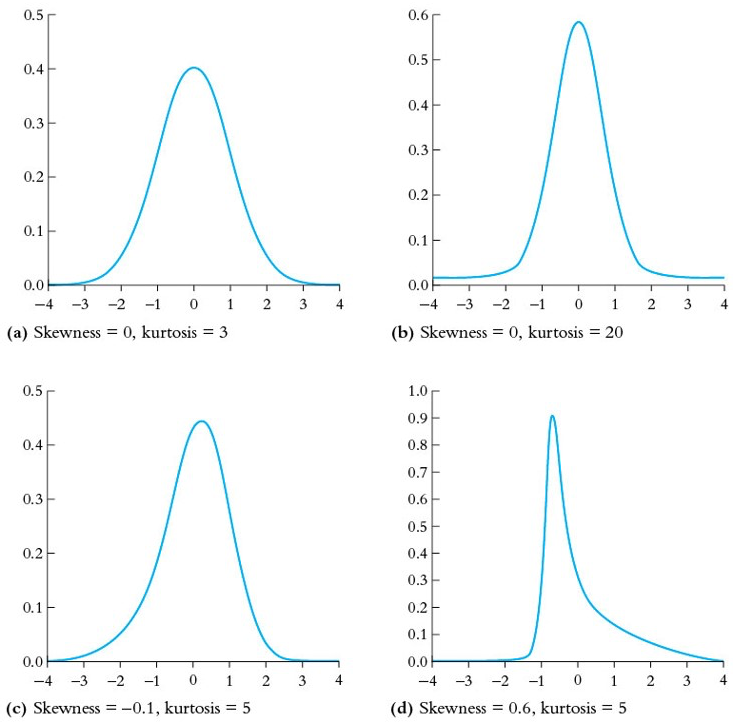
\includegraphics[scale=.6]{images/moments_examples.png}
\end{figure}
\end{column}
\end{columns}
\end{frame}


\section{Two Variables}

\begin{frame}{Joint Probability Distribution $Pr(X=x; Y=y)$}
 \begin{columns}
\begin{column}{0.45\textwidth}
Two dummy variables:
    \begin{itemize}
    \item $X = \{0;1\}$ --- Sunny Day (N/Y)
    \item $Y = \{0;1\}$ --- Ice Cream (N/Y)
    \end{itemize}
\vspace{.5cm}
Marginal Probability distribution:
\begin{equation*}
    Pr(Y=y) = \sum^k_{i=0} Pr(X=x_i; Y=y)
\end{equation*}
Conditional Probability distribution:
\begin{equation*}
    Pr(Y=y \mid X=x) = \frac{Pr(Y=y; X=x)}{Pr(X=x)}
\end{equation*}

\end{column}
\begin{column}{0.6\textwidth}
\vspace{1.2cm}
\begin{figure}
        \begin{table}
        \resizebox{.8\columnwidth}{!}{%
        \begin{tabular}{|c|c|c|c|}
        \hline
        Pr    & X=0 & X=1 & Total \\ \hline
        Y=0   & .15 & .25 & .4    \\ \hline
        Y=1   & .05 & .55 & .6    \\ \hline
        Total & .2  & .8  & 1     \\ \hline
        \end{tabular}%
        }
        \end{table}
\vspace{1cm}
\begin{eqnarray*}
    \Rightarrow Pr(Y=y; X=x) &= Pr(Y=y \mid X=x)Pr(X=x)\\
                             &= Pr(X=x \mid Y=y)Pr(Y=y)
\end{eqnarray*}
\end{figure}
\end{column}
\end{columns}
\end{frame}


\begin{frame}{Conditional and Iterated Expectations}
 \begin{columns}
\begin{column}{0.45\textwidth}
Two dummy variables:
    \begin{itemize}
    \item $X = \{0;1\}$ --- Sunny Day (N/Y)
    \item $Y = \{0;1\}$ --- Ice Cream (N/Y)
    \end{itemize}
\vspace{.5cm}
Conditional Expectation:
\begin{equation*}
    \mathbb{E}(Y\mid X=x)= \sum^k_{i=1} y_i  Pr(Y=y_i \mid X=x)
\end{equation*}
Iterated Expectation:
\begin{equation*}
    \mathbb{E}(Y)=\mathbb{E}[\mathbb{E}(Y\mid X=x)] \equiv \sum^k_{i=1} \mathbb{E}(Y\mid X=x_i) Pr(X=x_i)
\end{equation*}

\end{column}
\begin{column}{0.6\textwidth}
\begin{figure}
        \begin{table}
        \resizebox{.8\columnwidth}{!}{%
        \begin{tabular}{|c|c|c|c|}
        \hline
        Pr    & X=0 & X=1 & Total \\ \hline
        Y=0   & .15 & .25 & .4    \\ \hline
        Y=1   & .05 & .55 & .6    \\ \hline
        Total & .2  & .8  & 1     \\ \hline
        \end{tabular}%
        }
        \end{table}
\vspace{1cm}
\end{figure}
\end{column}
\end{columns}
\end{frame}


\begin{frame}{Independance}
    \begin{itemize}
        \item Two random variables $X$ and $Y$ are independent when the occurrence of one variable does not influence the value or affect the occurrence of the other.\vspace{.3cm}
    \end{itemize}
    \begin{eqnarray*}
        & Pr(Y=y\mid X=x)&= Pr(Y=y)\\
        \Leftrightarrow & Pr(Y=y; X=x)&= Pr(Y=y)Pr(X=x)
    \end{eqnarray*}
    \begin{itemize}
        \item  The joint probability distribution of $X$ and $Y$ can be expressed as the product of their individual probability distributions\vspace{.3cm}
        \item For example, think of the outcome of throwing two dice, $X$ and $Y$. 
    \end{itemize}
\end{frame}

\begin{frame}{Covariance}
    \begin{itemize}
        \item The covariance between $X$ and $Y$, $\sigma_{XY}$ or $cov(X,Y)$, is the average product of how two variables differ from their means. It measures how $X$ and $Y$ move together. 
    \end{itemize}
\begin{eqnarray*}
    &\sigma_{XY} &= \mathbb{E}[(X-\mathbb{E}(X))(Y-\mathbb{E}(Y))]\\
    &  &=\sum^k_{i=1}\sum^l_{j=1} (x_i-\mu_X)(y_j-\mu_Y)Pr(X=x_i; Y=y_j)
\end{eqnarray*} 
 \begin{itemize}
     \item A positive covariance suggests that when one variable is above its mean, the other tends to be above its mean too. When $X$ and $Y$ are independent, $\sigma_{XY}=0$.\vspace{.2cm}
    \item However, interpreting covariance is tricky due to scale differences... 
 \end{itemize}       
\end{frame}

\begin{frame}{Correlation}
 \begin{columns}
\begin{column}{0.45\textwidth}
    \begin{itemize}
    \item To clarify the relationship, covariance is normalized by the variables' standard deviations.
    \item This normalized coefficient is the correlation, $\rho_{XY}=\frac{\sigma_{XY}}{\sigma_{X}\sigma_{Y}}\in [-1; 1]$.
    \end{itemize}
\end{column}
\begin{column}{0.6\textwidth}
\begin{figure}
  \centering
         \vspace{-1mm}
        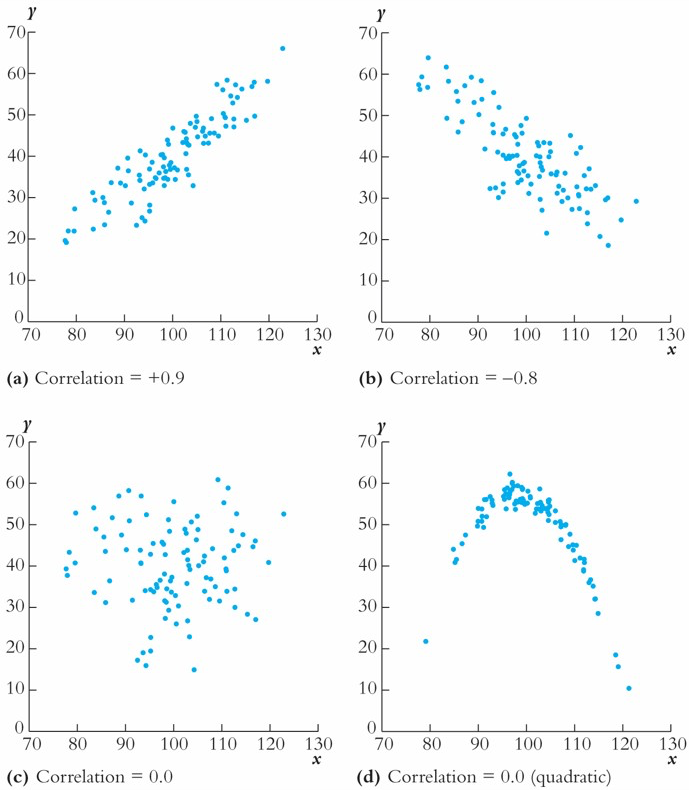
\includegraphics[scale=.56]{images/correlation_examples.png}
\end{figure}
\end{column}
\end{columns}
\end{frame}



\section{Random Sampling}

\begin{frame}{Random Sampling}
    \begin{itemize}
        \item In simple random sampling, $n$ objects ($y_1, y_2, ..., y_n$) are randomly drawn from a population (e.g., days, individuals, firms, etc.) such that each object has an equal and independent chance of being included in the sample\vspace{.2cm}
        \item It aims to form a representative sample to draw valid conclusions about the population's characteristics based on observed sample data.\vspace{.2cm}
        \item Because $y_1, y_2, ..., y_n$ are randomly drawn from the same population, the marginal distribution of $y_i$ is the same for each $i$:  $y_1, y_2, ..., y_n$ are identically distributed\vspace{.2cm}
        \item Because $y_1, y_2, ..., y_n$ are randomly drawn, knowing the value of $y_i$ does not provide information about $y_{j\neq i}$:  $y_1, y_2, ..., y_n$ are independently distributed\vspace{.2cm}
        \item When $y_1, y_2, ..., y_n$ are randomly drawn from the same distribution, they are independently and identically distributed (i.i.d.). Then, the expected value of every draw is the population mean, and so is the variance.
    \end{itemize}
\end{frame}


\begin{frame}{Sample Distribution Mean and Dispersion}
    \begin{itemize}
        \item Because the sample is drawn at random, the sample average (and other statistics), $\overline{Y}=\frac{1}{n}\sum^n_{i=1} y_i$, is also random.\vspace{.2cm}
        \item Because $\overline{Y}$ is random, it has a probability distribution. The distribution of $\overline{Y}$ is called the sampling distribution of $\overline{Y}$, i.e, it is the probability distribution associated with possible values of $\overline{Y}$ that could be computed for different random samples of size $n$.\vspace{.2cm}
        \item The expected value of the sampling distribution of $\overline{Y}$ is the population mean: $\mathbb{E}(\overline{Y})=\mu_Y$\vspace{.2cm}
        \item The variance of the sampling distribution of $\overline{Y}$ is:
    \end{itemize}
    \begin{eqnarray*}
        \sigma^2_{\overline{Y}} = var(\frac{1}{n}\sum^n_{i=1} y_i) =\frac{1}{n^2}\sum^n_{i=1} var(y_i) + \underbrace{\frac{1}{n^2}\sum^n_{i=1} \sum^n_{j=1;j\neq i} cov(y_i, y_j)}_{=0 ~~\text(because~i.i.d)} =\frac{1}{n}\sigma^2_Y 
    \end{eqnarray*}

    \begin{itemize}
        \item The standard deviation of the sampling distribution is therefore given by $\frac{\sigma_Y}{\sqrt{n}}$
    \end{itemize}
\end{frame}




\begin{frame}{Asymptotic properties ($n\rightarrow\infty$) of the sampling distribution (1/2)}
    \begin{itemize}
        \item If $y_1, y_2, ..., y_n$ are drawn randomly from the same population (i.i.d.) and large outliers are unlikely, then $\overline{Y}$ will approximate $\mathbb{E}(Y)$ as $n$ grows 
        \begin{itemize}
            \item In our previous example, the expected value for a sunny day is .8. If we were to randomly draw days from the entire history, the average number of sunny days converges to .8 as we draw more days from history.
            \item  If you flip it a lot of times, the average number of heads you get gets closer to 50\%, which is what we expect from a fair coin.
        \end{itemize}
        \item In this case, we say that $\overline{Y}$ converges in probability to $\mathbb{E}(Y)$
        \begin{itemize}
            \item The probability that $\overline{Y}$ equals $\mathbb{E}(Y)$ converges to 1 as $n$ grows (as $\lim_{n\rightarrow\infty}\sigma^2_{\overline{Y}}=0$)
        \end{itemize}
    \end{itemize}
    \begin{exampleblock}{(Weak) Law of Large Numbers}
        If $y_i$ are independent and identically distributed and $\mid \mathbb{E}(Y)\mid<\infty$, then as $n\rightarrow\infty$,
        \begin{equation*}
            \overline{Y}=\frac{1}{n}\sum^n_{i=1} y_i\xrightarrow{\mathit{p}}\mathbb{E}(Y)\equiv\mu_Y
        \end{equation*}
    \end{exampleblock}
\end{frame}


\begin{frame}{Example -- tossing a coin}
    \begin{center}
        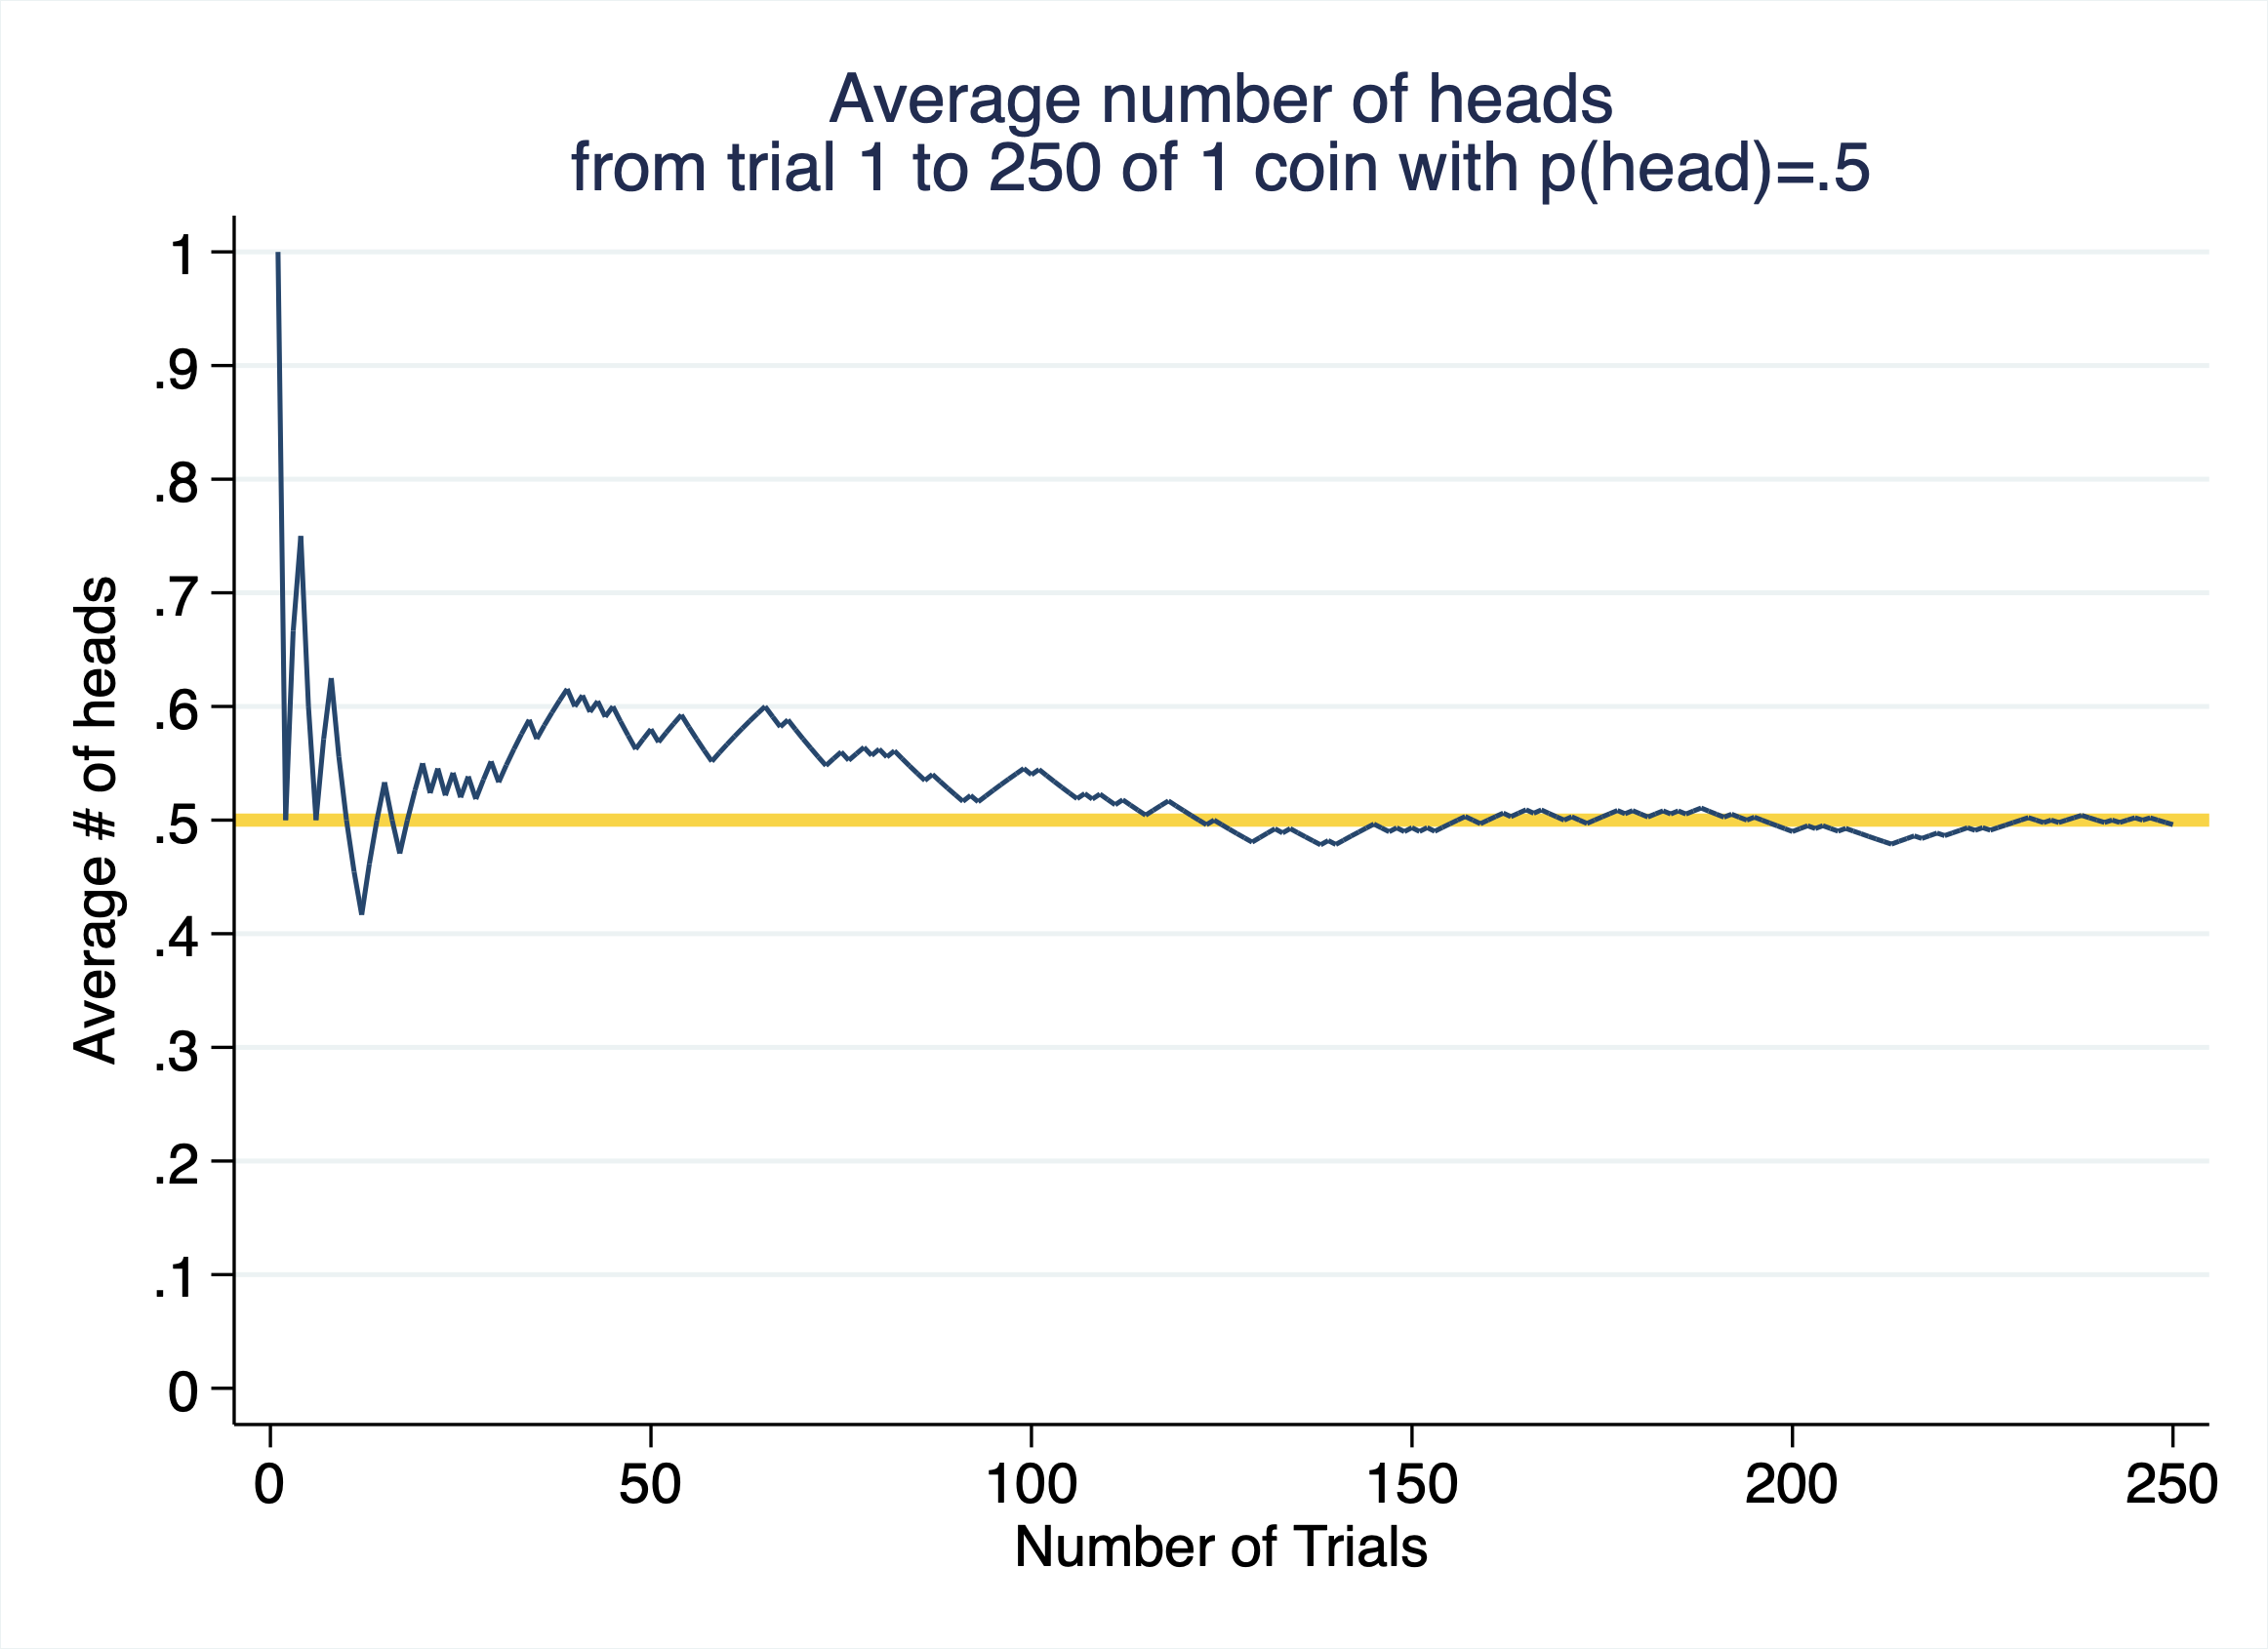
\includegraphics[scale=.25]{images/heads.png}
    \end{center}
\end{frame}


\begin{frame}{Asymptotic properties ($n\rightarrow\infty$) of the sampling distribution (2/2)}
    \begin{itemize}
        \item Random sample averages behave in a predictable pattern.
        \item If $y_1, y_2, ..., y_n$ are drawn randomly from the same population (i.i.d.) and large outliers are unlikely, then $\overline{Y} \sim \mathcal{N}(\mu_Y, \sigma^2_{\overline{Y}})$ as $n$ grows
        \begin{itemize}
            \item When you randomly gather a large group of people from UPF and calculate their average height, repeating this with many groups, the resulting sample averages distribution will form a bell-shaped curve, regardless of the actual height distribution at UPF.
        \end{itemize}
        \item $\overline{Y} \sim \mathcal{N}(\mu_Y, \sigma^2_{\overline{Y}})$ exactly when $Y \sim \mathcal{N}(\mu_Y, \sigma^2_Y)$, and approximately when $Y$ follows another distribution
        \item Very powerful because it allows us to make better predictions and draw conclusions about populations based on smaller samples
    \end{itemize}
    \begin{exampleblock}{Central Limit Theorem}
        If $y_i$ are independent and identically distributed and $0<\sigma^2_Y<\infty$, then as $n\rightarrow\infty$,
        \begin{equation*}
            \frac{\overline{Y}-\mu_Y}{\sigma_{\overline{Y}}} \sim \mathcal{N}(0, 1)
        \end{equation*}
    \end{exampleblock}
\end{frame}


\begin{frame}{Example -- tossing a coin ($n=100$ flips, 10K times)}
    \begin{center}
        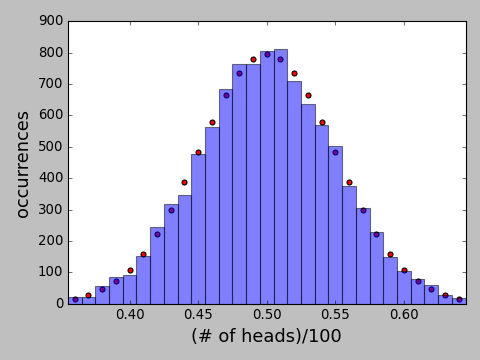
\includegraphics[scale=.55]{images/clt_heads.png}
    \end{center}
\end{frame}


\section{Estimation}
\begin{frame}{Estimators}
\begin{itemize}
    \item Imagine you do not know $\mu_Y$ and want to \textit{estimate} it. The sample average $\overline{Y}$ is a natural way to estimate $\mu_Y$, but not the only one
    \begin{itemize}
        \item NB: $Y_1$, $Y_3$, $Y_2/5$... All can be estimators of $\mu_Y$
    \end{itemize}
    \item An estimator is a \textit{function} of sample data drawn randomly from the population. It is random because of the randomness of the random sampling process.
    \item An estimate is the \textit{numerical value} of an estimator taken from a given sample. It is a non-random number.
    \item How to determine if an estimator is better than another? Let $\hat{\mu}_y$ and $\tilde{\mu}_y$ be two estimators of $\mu_Y$.
    \begin{enumerate}
        \item $\hat{\mu}_y$ is \textit{unbiased} if $\mathbb{E}(\hat{\mu}_y) = \mu_Y$
        \item $\hat{\mu}_y$ is \textit{consistent} if $\hat{\mu}_y \xrightarrow{\mathit{p}}\mu_Y$
        \item $\hat{\mu}_y$ is \textit{more efficient}  than $\tilde{\mu}_y$ if $\operatorname{var}(\hat{\mu}_y) = \operatorname{var}(\tilde{\mu}_y)$
    \end{enumerate}
\end{itemize}
\end{frame}

\begin{frame}{Is your estimator BLUE?}
\begin{itemize}
    \item $\overline{Y}$ is an estimator of  $\mu_Y$ which is:
    \begin{enumerate}
        \item \textit{Unbiased} : $\mathbb{E}(\overline{Y}) = \mu_Y$
        \item \textit{Consistent} : $\overline{Y}\xrightarrow{\mathit{p}}\mu_Y$
        \item \textit{(Most) Efficient}: \begin{eqnarray*}
        & var(\hat{\mu}_y)\geq \mathbb{I}_{\mu_Y}^{-1} = \frac{\sigma_Y}{n} &\text{\small (Cramer-Rao Inequality + Central Limit Theorem)}\\
        & \Leftrightarrow var(\hat{\mu}_y)\geq var(\overline{Y})
        \end{eqnarray*}
    \end{enumerate}
    \item $\overline{Y}$ is the \textbf{B}est \textbf{L}inear \textbf{U}nbiased \textbf{E}stimator of  $\mu_Y$
    \begin{itemize}
        \item i.e., it is the most efficient estimator of all estimators which are a linear function of $Y_1\dots Y_n$.
    \end{itemize}
    \item What estimator $\hat{\mu}_y$ minimizes the sum of the squared distance between $Y_i$ observations?
        \begin{eqnarray*}
            \frac{\partial}{\partial\hat{\mu}_y} \sum_{i=1}^n (Y_i- \hat{\mu}_y)^2 &=0\\
           \Leftrightarrow -2\sum_{i=1}^n (Y_i- \hat{\mu}_y)&=0\\
           \Leftrightarrow \overline{Y}&=\hat{\mu}_y & \text{($\overline{Y}$ is the least square estimator of $\mu_Y$)}\\
        \end{eqnarray*}
    \end{itemize}
\end{frame}


\begin{frame}[allowframebreaks]{Material}
\begin{itemize}
    \item[--] \textbf{Textbooks:}
    \begin{itemize}
        \item Introduction to Econometrics, 4th Edition, Global Edition, by Stock and Watson -- Chapters 1 - 2
    \end{itemize}
\end{itemize}
\end{frame}



\end{document}
